%analyse + méthodo
Nous avons très rapidement choisi de réaliser notre TER avec une méthode agile, SCRUM, car, en plus d'être aujourd'hui de plus en plus utilisée en entreprise, elle nous permettait d'avoir une version de notre projet fonctionnelle à la fin de chaque sprint.

Lors du sprint 0, nous avons effectué une analyse des outils à notre disposition (Flex, Bison, etc) et de l'existant, le langage Logo et ses dérivés, et avons réalisé une estimation du temps de travail (cf.~\ref{planning}) pour évaluer combien de sprints nous pourrions faire en prenant compte des autres activités parallèles (cours, examens, révisions, etc.).
\begin{figure}[h]
\caption{\label{planning} Planning OpenProject}
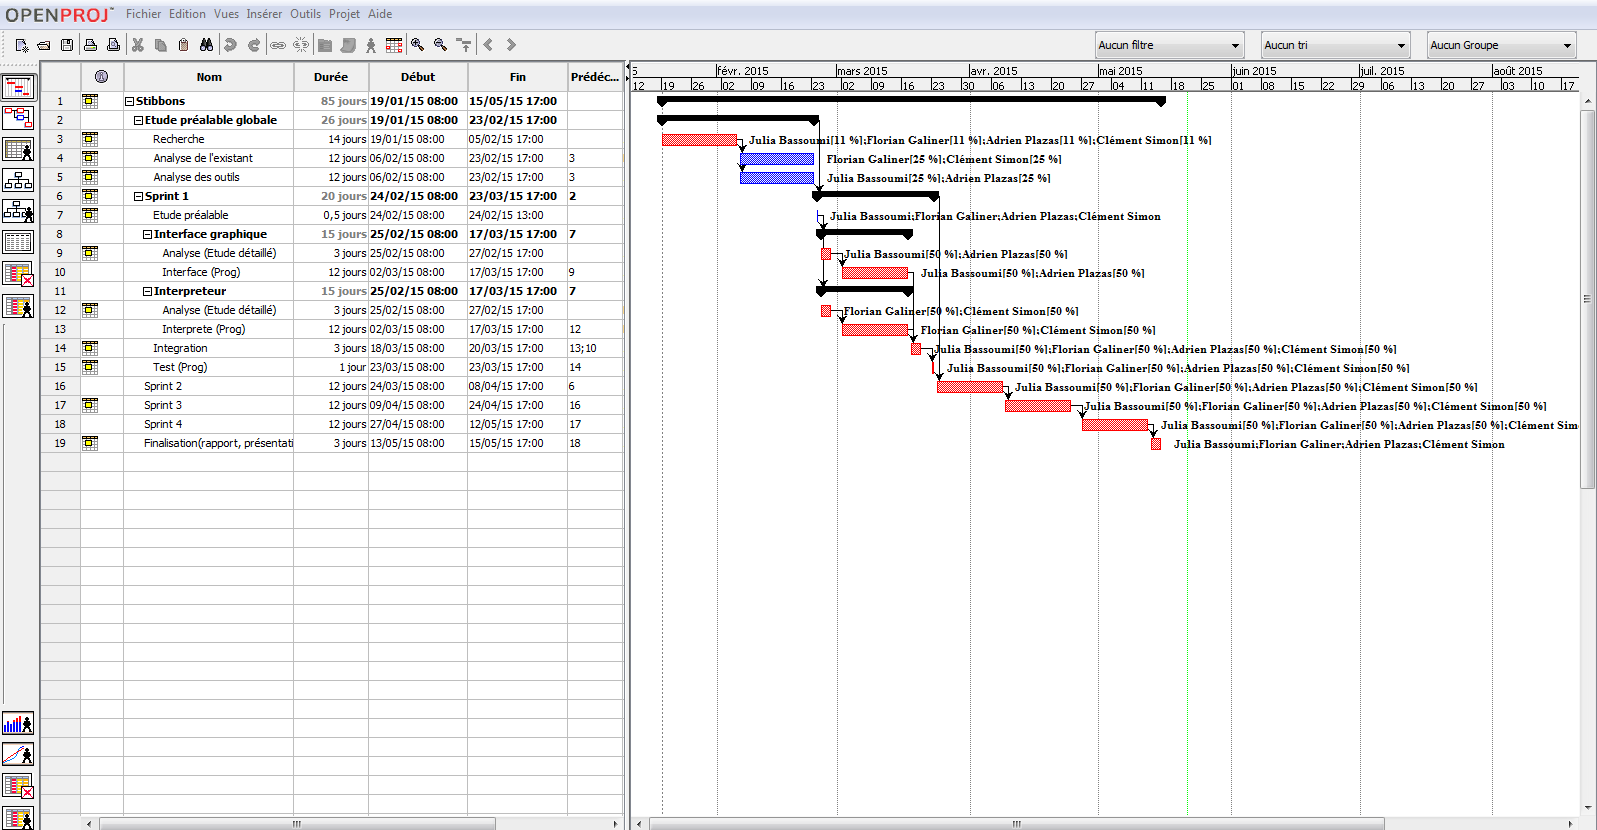
\includegraphics[scale=0.35]{doc/gestionProjet/planning.PNG}
\end{figure}

Après réunion avec notre encadrant, nous avons également défini les différentes fonctionnalités (sous forme de scénarios utilisateurs) que nous souhaitions voir dans notre future application, associant à chacune d'entre elles une priorité, et avons établi à partir de là notre backlog initial (cf. Table~\ref{bsp1}).

%Nous avons développé à la manière d'un développement interne en entreprise, il n'y avait pas de client externe, puisque nous avions proposé notre projet.
Le projet a été développé semblablement à un projet interne d'entreprise. En effet, notre encadrant ne jouait pas le rôle d'un client mais plutôt celui d'un patron.

Nous effectuions une réunion en début de chaque sprint, au cours de laquelle nous commencions par choisir les tâches devant être réalisées durant le sprint selon leurs priorités, mais également selon d'autres facteurs (ordre de réalisation, temps de travail, etc). 

L'estimation du volume horaire nécessaire à chaque sprint était réalisée à l'aide de petits papiers. Chacun de nous mettait ses estimations minimale et maximale que nous mettions en commun avant d'en discuter. L'estimation finale correspondait à la moyenne entre la plus haute et la plus petite de toutes les estimations. 

Lors du premier sprint, nous nous sommes réparti le travail selon les envies de chacun. Il est cependant vite apparu que deux groupes de deux personnes ressortaient~: un groupe centré sur le modèle et l'interface et un groupe centré sur la grammaire et l'interprète. 
À chaque sprint, chacun avait une ou plusieurs tâches à effectuer, parfois seul, parfois en collaboration.

{\tiny
\begin{longtable}[c]{|c|p{2cm}|c|p{4cm}|*{4}{c|}}
\hline
\bf id & \bf Scénario utilisateur & \bf Priorité & \bf Tests & \bf Estimation & \bf Sprint & \bf Statut & \bf Temps réel \\
\hline
\endfirsthead
\hline
\bf id & \bf Scénario utilisateur & \bf Priorité & \bf Tests & \bf Estimation & \bf Sprint & \bf Statut & \bf Temps réel \\
\hline
\endhead
\hline
\caption{Backlog Initial.} \label{bsp1}\\
\endlastfoot
\hline
\caption[]{Backlog Initial.}\\
\endfoot
1 & L'utilisateur écrit du code dans un éditeur & 200 &  &  &  &  &  \\
\hline
2 & L'utilisateur importe du code dans le logiciel & 1100 & Importer du code Stibbons depuis un fichier, vérifier que le code obtenu est bien identique à celui du fichier. & 4h & 1 & Fini & 1h \\
\hline
3 & L'utilisateur visualise les rapports d'erreurs du code & 400 &  &  &  &  &  \\
\hline
4 & L'utilisateur visualise l'évolution du modèle & 1400 & Vérifier que l'interprétation d'instructions données fait bien évoluer comme prévu la tortue dans son environnement. & 24h & 1 & Fini & 70h \\
\hline
5 & L'utilisateur modifie la vitesse (pause, pas à pas, parallèle) & 700 &  &  &  &  &  \\
\hline
6 & Le «~dieu-tortue~» interprète le code de l'utilisateur & 1500 & Lancer l'interprétation pour~: repeat 4 { fd 1 rt 90 } (suivant syntaxe) ainsi que pour du code avec des erreurs~: repat 4 {...} par exemple ou repeat 4 { fd 1 rt } & 12h & 1 & Fini & 32h \\
\hline
7 & L'utilisateur crée une nouvelle tortue (avec un code) & 600 & Lancer l'interprétation pour~: create-turtle {} et observer une nouvelle tortue apparaître dans l'interface graphique. & 7,5h & 2 &  &  \\
\hline
8 & Les tortues s'exécutent en parallèles & 1200 & Lancer l'interprétation pour deux tortues d'un bout de code et observer l'exécution parallèle via des écritures dans le terminal (Je suis tortue 1 et Je
suis tortue 2 par exemple) & 42,5h & 2 & & \\
\hline
9 & Les tortues communiquent directement entre elles & 900 &  &  &  &  &  \\
\hline
10 & Une tortue se déplace dans l'environnement & 1300 & Ecriture d'instructions simples~: repeat 4 { fd 1 rt 90 } (suivant syntaxe) - Renvoi de la position de la tortue après chaque deplacement~: where\_am\_i(); (suivant syntaxe) & 16h & 1 & Fini & 24h \\
\hline
11 & Les tortues communiquent avec les zones de l'environnement & 1000 &  &  &  &  &  \\
\hline
12 & L'utilisateur exporte le code & 500 &  &  &  &  &  \\
\hline
13 & L'utilisateur exporte le modèle & 300 &  &  &  &  &  \\
\hline
14 & L'utilisateur ajoute une entrée & 100 &  &  &  &  &  \\
\hline
15 & L'utilisateur remet à zéro l'environnement & 800 &  &  &  &  &  \\
\hline
16 & L'utilisateur utilise des variables dans le code & 1275 & Ecrire a = 90 fd a et observer la tortue qui avance. & 12h & 2 &  &  \\
\hline
17 & L'utilisateur définit des fonctions personnalisées dans le code & 1250 & Ecrire function f () { fd 90 } f () et observer la tortue qui avance. & 23,5h & 2 & &  \\
\hline
18 & Les tortues communiquent via l'environnement & 950 &  &  &  &  &  \\
\hline
19 & L'utilisateur utilise des conditionnelles & 550 & Ecrire if(false) { fd 90 } et observer que la tortue ne bouge pas. Refaire le même test avec if(true) et observer que la tortue bouge. & 3,5h & 2 &  &  \\
\hline
20 & L'utilisateur utilise des boucles & 575 & Ecrire pd repeat 4 { fd 40 rt 90 } et observer que la tortue dessine un carré. & 7h & 2 &  &  \\
\hline
\end{longtable}}
